\documentclass[10pt,a4paper]{article}

% --- Packages ---
\usepackage[utf8]{inputenc}
\usepackage[T1]{fontenc}
\usepackage[spanish,es-nodecimaldot]{babel}
\usepackage{amsmath,amssymb,amsfonts}
\usepackage{graphicx}
\usepackage{booktabs}
\usepackage{tabularx}
\usepackage{array}
\usepackage[margin=2.2cm,top=2.5cm,bottom=2.5cm]{geometry}
\usepackage{xcolor}
\usepackage{microtype}
\usepackage{enumitem}
\usepackage{caption}
\usepackage{titlesec}
\usepackage{fancyhdr}
\usepackage{tikz}
\usetikzlibrary{shapes,arrows.meta,positioning,calc}

% --- Colors ---
\definecolor{primaryblue}{RGB}{2, 132, 199}
\definecolor{darkslate}{RGB}{15, 23, 42}
\definecolor{accentblue}{RGB}{3, 105, 161}
\definecolor{lightbg}{RGB}{248, 250, 252}
\definecolor{borderline}{RGB}{226, 232, 240}
\definecolor{alertred}{RGB}{185, 28, 28}

% --- Hyperref ---
\usepackage[
    colorlinks=true,
    linkcolor=accentblue,
    citecolor=primaryblue,
    urlcolor=accentblue,
    bookmarks=true
]{hyperref}

% --- Header & Footer ---
\pagestyle{fancy}
\fancyhf{}
\fancyhead[L]{\small \textcolor{gray}{cellSim Working Paper 2026-01: Inferencia Bayesiana Canónica y Validación Secundaria}}
\fancyhead[R]{\small \textcolor{gray}{Equipo cellSim}}
\fancyfoot[C]{\thepage}
\renewcommand{\headrulewidth}{0.4pt}
\renewcommand{\footrulewidth}{0pt}

% --- Section Styling ---
\titleformat{\section}
  {\normalfont\Large\bfseries\color{darkslate}}{\thesection}{1em}{}[\color{primaryblue}\titlerule]
\titleformat{\subsection}
  {\normalfont\large\bfseries\color{accentblue}}{\thesubsection}{1em}{}
\titleformat{\subsubsection}
  {\normalfont\normalsize\bfseries\color{darkslate}}{\thesubsubsection}{1em}{}

\setlist[itemize]{leftmargin=1.8em, itemsep=0.2em, topsep=0.3em}
\setlist[enumerate]{leftmargin=1.8em, itemsep=0.2em, topsep=0.3em}
\setlist[description]{leftmargin=2.2em, itemsep=0.4em, topsep=0.4em, font=\bfseries\color{accentblue}}

\begin{document}

% --- Title & Header Metadata ---
\begin{center}
    {\LARGE \textbf{\color{darkslate} cellSim Working Paper 2026-01: Evaluación de Sensibilidad Global de Parámetros Secundarios, Reducción de Varianza Multivariante y Dinámica Fisiológica TP53/BRCA1}} \\[0.8em]
    {\large \textbf{Autores:} Equipo cellSim} \\[0.3em]
    {\normalsize \textbf{Fecha:} 28 de agosto de 2026 \quad $\vert$ \quad \textbf{Clasificación:} Biología Teórica, Oncología Matemática, Inferencia Bayesiana (ABC-SMC)}
\end{center}

\vspace{0.5em}
\hrule height 1pt
\vspace{1em}

% --- Abstract ---
\begin{abstract}
\noindent
En este documento de trabajo se analiza la robustez estructural, la identificabilidad bayesiana y la resiliencia del modelo estocástico multiescala basado en agentes \textbf{cellSim} ante la relajación simultánea de los parámetros que permanecieron fijos en su calibración original. Mediante un protocolo de \textit{Approximate Bayesian Computation} acoplado a \textit{Sequential Monte Carlo} (ABC-SMC) estructurado en tres niveles crecientes de libertad e incertidumbre ($\pm10\%$, $\pm25\%$ y $\pm50\%$), se evalúa la contracción del espacio posterior frente a la cohorte epidemiológica de referencia de portadoras de $BRCA1^{+/-}$ (\textit{Kuchenbaecker et al., JAMA 2017}).

\vspace{0.5em}
\noindent Demostramos que:
\begin{enumerate}
    \item \textbf{Dominancia de Parámetros Primarios:} La tasa de mutación somática del segundo alelo de $BRCA1$ ($\beta_{BRCA1}$) y el coeficiente de inestabilidad con $BRCA1$ activo ($\delta_{\text{BRCA+}}$) concentran la práctica totalidad de la identificabilidad bayesiana, contrayendo sus intervalos de credibilidad al 95\% a una fracción estrecha del prior ($\beta_{BRCA1} = 0.0459 \pm 0.0041$ [$95\%\text{ CI: } 0.0381, 0.0535$] y $\delta_{\text{BRCA+}} = 0.1067 \pm 0.0164$ [$95\%\text{ CI: } 0.0795, 0.1403$]).
    \item \textbf{Naturaleza de Parámetros \textit{Sloppy} (Blandos):} Los parámetros secundarios ($\theta_{D\text{\_intr}}$, $\theta_{D\text{\_inmune}}$, $d_{\text{basal}}$, $\phi_{\text{tumor}}$) presentan distribuciones posteriores planas que abarcan la totalidad del soporte a priori con centros de gravedad invariantes en sus valores originales $\theta_0$. Esto demuestra matemáticamente que los datos epidemiológicos clínicos agregados no restringen sus valores individuales y que fijarlos en el diseño base responde estrictamente al principio de parsimonia (Navaja de Ockham).
    \item \textbf{El Gen TP53 como Interruptor Fisiológico On/Off:} A diferencia de $BRCA1$ (cuya tasa $\beta_{BRCA1}$ modula continuamente la latencia clínica), la tasa de degradación de $TP53$ ($\mu_{TP53} = 0.0030$) actúa como una condición de frontera biológica crítica: un incremento de apenas $+0.0005$ destruye la meseta clínica del $\approx 70\%$ de penetrancia acumulada a los 80 años observada en pacientes humanas, disparando el error cuadrático global ($SSE$) en un $+1200\%$.
    \item \textbf{Estabilidad de Fenotipos Tumorales:} La estructura bimodal de dos subtipos tumorales emergentes---\textbf{Fenotipo A (Escape Proliferativo Clonal / Alta Proliferación)} y \textbf{Fenotipo B (Contención Tisular / Basal-Resiliente)}---se mantiene invariante en los niveles fisiológicos de incertidumbre ($\pm10\%$ y $\pm25\%$), colapsando únicamente en el nivel extremo ($\pm50\%$) por inducción de ruido blanco estocástico derivado de la sobre-parametrización.
\end{enumerate}
\end{abstract}

\vspace{1em}
\hrule height 0.5pt
\vspace{1.5em}

% --- Section 1 ---
\section{Introducción y Marco del Modelo}

\subsection{Contexto Biológico y Definición del Modelo Agentic Cell}

La carcinogénesis mamaria en pacientes portadoras de mutaciones germinales heterocigotas en el gen $BRCA1$ ($BRCA1^{+/-}$) representa un proceso biológico gobernado por la interacción estocástica entre la pérdida de función de reparación genómica, la vigilancia apoptótica y la capacidad de evasión del microambiente celular.

El simulador \textbf{cellSim} modela este proceso mediante el paradigma de \textbf{Células Agénticas (\textit{Agentic Cells})}, donde cada célula del tejido epitelial actúa como un agente computacional autónomo con estado interno, ciclo de vida secuencial y toma de decisiones probabilística basada en umbrales de daño.

\begin{center}
\begin{tikzpicture}[
    node distance=1.8cm,
    state/.style={rectangle, rounded corners, draw=darkslate, fill=lightbg, thick, inner sep=6pt, align=center, font=\small},
    dead/.style={rectangle, rounded corners, draw=alertred, fill=red!10, thick, inner sep=6pt, align=center, font=\small},
    arrow/.style={-Latex, thick, darkslate}
]
    \node[state] (s0) {\textbf{[BASELINE]}\\$BRCA1: +/-$\\$TP53: +/+$\\(Sano/Estable)};
    \node[state, right=0.8cm of s0] (s1) {\textbf{[UNSTABLE]}\\$BRCA1: +/-$\\$TP53: +/-$\\(Daño Leve)};
    \node[state, right=0.8cm of s1] (s2) {\textbf{[UNPROTECTED]}\\$BRCA1: +/-$\\$TP53: -/-$\\(Sin Freno p53)};
    \node[state, right=0.8cm of s2] (s3) {\textbf{[PRIMER]}\\$BRCA1: -/-$\\$D_{\text{intr}} \ge \theta_{D\text{\_intr}}$\\(Pre-tumoral)};
    \node[state, right=0.8cm of s3] (s4) {\textbf{[TUMORAL]}\\$BRCA1: -/-$\\$D_{\text{inm}} \ge \theta_{D\text{\_inmune}}$\\(Evasión Inmune)};

    \node[dead, below=1.2cm of s0] (d0) {\textbf{[DEAD]}\\Apoptosis p53};
    \node[dead, below=1.2cm of s1] (d1) {\textbf{[DEAD]}\\Apoptosis p53};

    \draw[arrow] (s0) -- node[above, font=\footnotesize] {$\mu_{TP53}$} (s1);
    \draw[arrow] (s1) -- node[above, font=\footnotesize] {$\mu_{TP53}$} (s2);
    \draw[arrow] (s2) -- node[above, font=\footnotesize] {$\beta_{BRCA1}$} (s3);
    \draw[arrow] (s3) -- node[above, font=\footnotesize] {$\delta_{\text{BRCA-}}$} (s4);

    \draw[arrow, alertred] (s0) -- node[right, font=\footnotesize] {Si BRCA1 muta $-/-$} (d0);
    \draw[arrow, alertred] (s1) -- node[right, font=\footnotesize] {Si BRCA1 muta $-/-$} (d1);
\end{tikzpicture}
\end{center}

\vspace{0.5em}
\noindent\colorbox{red!8}{\parbox{\dimexpr\textwidth-2\fboxsep\relax}{
\small \textbf{\color{alertred} Regla Biológica Fundamental de Viabilidad:} Si una célula en estado \texttt{BASELINE} ($TP53^{+/+}$) o \texttt{UNSTABLE} ($TP53^{+/-}$) experimenta la pérdida somática del segundo alelo de $BRCA1$ ($BRCA1^{+/-} \to BRCA1^{-/-}$), \textbf{la célula es eliminada inmediatamente por apoptosis (transición directa a \texttt{DEAD})}. La presencia de proteína p53 funcional detecta el colapso en la recombinación homóloga e induce el suicidio celular. Para que una célula con daño severo en $BRCA1$ sobreviva y progrese hacia la malignidad, \textbf{es requisito biológico \textit{sine qua non} que $TP53$ haya mutado previamente a $-/-$ (\texttt{UNPROTECTED})}.
}}
\vspace{0.8em}

Cada célula está caracterizada formalmente por cuatro variables de estado y dos umbrales críticos de activación:

\begin{description}
    \item[Estado Génico $BRCA1$:] Gen supresor tumoral responsable de la reparación de roturas de doble cadena de ADN por recombinación homóloga.
    \begin{itemize}
        \item \textit{Estado nativo:} $BRCA1^{+/-}$ (heterocigoto, funcional, vivo).
        \item \textit{Transición:} Mutación somática unidireccional del segundo alelo $BRCA1^{+/-} \to BRCA1^{-/-}$ con tasa probabilística anual $\beta_{BRCA1}$ (\texttt{brca1\_rate}).
        \item \textit{Regla de letalidad sintética:} Una célula $BRCA1^{-/-}$ en presencia de $TP53$ funcional es detectada y sufre apoptosis inmediata (\texttt{DEAD}). Solo si $TP53$ ha perdido su función ($-/-$), la célula $BRCA1^{-/-}$ sobrevive, acumulando daño genómico acelerado.
    \end{itemize}

    \item[Estado Génico $TP53$:] El guardián del genoma, mediador maestro de la parada del ciclo celular y de la apoptosis intrínseca.
    \begin{itemize}
        \item \textit{Estados posibles:} $+/+$ (homocigoto funcional), $+/-$ (heterocigoto con función parcial), $-/-$ (nulo / deficiente).
        \item \textit{Transición:} Progresión mutacional estocástica $+/+ \to +/- \to -/-$ regida por la tasa base $\mu_{TP53}$ (\texttt{tp53\_rate}).
    \end{itemize}

    \item[Acumulador $D_{\text{intr}}$ y Umbral $\theta_{D\text{\_intr}}$ (Daño ADN Intrínseco):] Variable continua adimensional que cuantifica la carga de daño macromolecular y aberraciones cromosómicas acumuladas:
    \begin{equation}
        D_{\text{intr}}(t+1) = D_{\text{intr}}(t) + \delta_{\text{intr}}(t) + \text{age\_factor}(t)
    \end{equation}
    \textbf{Umbral $\theta_{D\text{\_intr}} = 2.0$ (Barrera de Inestabilidad Intrínseca):} Punto de corte biofísico a partir del cual el daño supera la capacidad basal de reparación celular. Cuando $D_{\text{intr}} \ge \theta_{D\text{\_intr}}$ bajo fondo $TP53^{-/-}$, la célula transiciona al estado \textbf{PRIMER} (célula pre-neoplásica detectable por el microambiente).

    \item[Acumulador $D_{\text{inm}}$ y Umbral $\theta_{D\text{\_inmune}}$ (Resistencia Inmune / Evasión Extrínseca):] Variable continua adimensional que mide el grado de inmunorresistencia y la capacidad de anular las señales pro-apoptóticas del estroma:
    \begin{equation}
        D_{\text{inm}}(t+1) = D_{\text{inm}}(t) + \delta_{\text{inm}}(t) + \text{age\_factor}(t)
    \end{equation}
    \textbf{Umbral $\theta_{D\text{\_inmune}} = 5.0$ (Barrera de Evasión Extrínseca / Inmune):} Punto de corte biológico que representa la neutralización de la vigilancia inmune. Cuando $D_{\text{inm}} \ge \theta_{D\text{\_inmune}}$, la célula transiciona al estado \textbf{TUMORAL} (inmortalización celular, evasión de apoptosis extrínseca y desregulación proliferativa).
    \textbf{Ratio de Barrera $\theta_{D\text{\_inmune}} / \theta_{D\text{\_intr}} = 2.5$:} Esta asimetría formaliza que alcanzar la evasión inmune sostenida requiere $2.5\times$ más acumulación biológica que franquear la inestabilidad genómica intrínseca inicial.
\end{description}

\subsection{Resumen de la Calibración Previa ABC-SMC y Comparación Epidemiológica}

En la calibración fundamental de \textbf{cellSim}, el modelo fue parametrizado frente a la mayor cohorte clínica prospectiva de portadoras de $BRCA1$: el estudio de \textbf{Kuchenbaecker et al. (JAMA 2017)} ($N=9.856$ portadoras). A continuación, se presenta la comparación entre la incidencia acumulada observada en la población general y en portadoras de $BRCA1^{+/-}$:

\begin{table}[h!]
\centering
\small
\caption{\textbf{Tabla Comparativa de Incidencia Acumulada de Cáncer de Mama por Edad: Población General vs. Cohorte BRCA1}}
\begin{tabular}{ccc}
\toprule
\textbf{Edad (Años)} & \textbf{IAPC (\%)} & \textbf{IACB (\%)} \\
\midrule
\textbf{20} & $0.00\%$ & $0.00\%$ \\
\textbf{30} & $0.08\%$ & $4.00\%$ \\
\textbf{40} & $0.59\%$ & $26.00\%$ \\
\textbf{50} & $2.23\%$ & $46.00\%$ \\
\textbf{60} & $4.80\%$ & $58.00\%$ \\
\textbf{70} & $8.14\%$ & $65.00\%$ \\
\textbf{80} & $11.18\%$ & $70.00\%$ \\
\bottomrule
\end{tabular}
\label{tab:incidencia_comparada}
\vspace{0.4em}
\begin{flushleft}
\footnotesize \textit{Definición de siglas y fuentes:} \textbf{IAPC}: Incidencia Acumulada en Población General (\textit{SEER / DevCan Database; Cancer Research UK}). \textbf{IACB}: Incidencia Acumulada en Cohorte $BRCA1^{+/-}$ (\textit{Kuchenbaecker et al., JAMA 2017}, vector objetivo $\mathbf{y}_{\text{obs}}$ empleado en cellSim).
\end{flushleft}
\end{table}

Dado que la función de verosimilitud analítica $p(\mathbf{y}_{\text{obs}} \mid \theta)$ de un sistema estocástico de 500 células interactuando durante 80 años es intratable, se empleó \textbf{Approximate Bayesian Computation acoplado a Sequential Monte Carlo (ABC-SMC)} (\textit{Toni et al., 2009; Liepe et al., 2014}).

\vspace{0.5em}
\noindent\textbf{Resultados Clave de la Calibración Base y Premisa de Parámetros Secundarios:}
\begin{enumerate}
    \item \textbf{Identificación de Parámetros Primarios:} Se obtuvieron distribuciones a posteriori estrechas para: $\beta_{BRCA1} = 0.0445 \pm 0.0041$ (tasa somática en $BRCA1$, $\sim 4.45\%$ anual), $\delta_{\text{BRCA+}} = 0.1093 \pm 0.0189$ (inestabilidad con $BRCA1$ activo / heterocigoto), y $d_{\text{neo}} = 0.1564 \pm 0.0410$ (tasa de proliferación clonal neoplásica).
    \item \textbf{Estructura Bimodal y Subtipos de Crecimiento:} Se descubrió una fuerte anticorrelación lineal ($r = -0.609$, $p < 10^{-21}$) entre $\delta_{\text{BRCA+}}$ y $d_{\text{neo}}$, que refleja dos estrategias celulares distintas:
    \begin{itemize}
        \item \textbf{Fenotipo A (Escape Proliferativo Clonal / Rápida Expansión):} $\delta_{\text{BRCA+}} \approx 0.095, d_{\text{neo}} \approx 0.189$. Barrera apoptótica más laxa con colonización rápida tras el escape.
        \item \textbf{Fenotipo B (Contención Tisular / Basal-Resiliente):} $\delta_{\text{BRCA+}} \approx 0.116, d_{\text{neo}} \approx 0.133$. Mayor contención estromal con acumulación lenta y difusa de daño tisular.
    \end{itemize}
    \item \textbf{Identificación Empírica de Parámetros Secundarios:} Para garantizar la identificabilidad numérica y evitar el sobreajuste en 9 dimensiones, se fijaron empíricamente 5 parámetros secundarios: $\mu_{TP53} = 0.0030$, $\theta_{D\text{\_intr}} = 2.0$, $\theta_{D\text{\_inmune}} = 5.0$, $d_{\text{basal}} = 0.0010$ y $\phi_{\text{tumor}} = 0.05$.
\end{enumerate}

% --- Section 2 ---
\section{Diseño del Experimento de Sensibilidad Multinivel}

\subsection{Planteamiento del Problema: Identificabilidad y la Navaja de Ockham}

Cuando el número de parámetros libres crece excesivamente frente a la dimensionalidad de las observaciones clínicas disponibles (6 puntos de incidencia acumulada a lo largo de 80 años), los algoritmos de inferencia bayesiana caen en \textbf{variedades degeneradas (\textit{sloppy manifolds})}. En tales regiones, infinitas combinaciones arbitrarias generan curvas macroscópicamente indistinguibles (\textit{Gutenkunst et al., 2007; Transtrum et al., 2015}).

Para verificar cuantitativamente qué ocurre cuando todos los parámetros varían libremente, se diseñó un protocolo de tres niveles de incertidumbre:
\begin{itemize}
    \item \textbf{Nivel 1: Margen Fisiológico ($\pm10\%$):} Modela la incertidumbre y ruido de medición biológica ($\mu_{TP53} \in [0.0027, 0.0033]$, $\theta_{D\text{\_intr}} \in [1.8, 2.2]$, $\theta_{D\text{\_inmune}} \in [4.5, 5.5]$, etc.).
    \item \textbf{Nivel 2: Incertidumbre Intermedia ($\pm25\%$):} Modela variabilidad biológica interindividual moderada ($\mu_{TP53} \in [0.00225, 0.00375]$, $\theta_{D\text{\_intr}} \in [1.5, 2.5]$, etc.).
    \item \textbf{Nivel 3: Relajación Extrema ($\pm50\%$):} Prueba de estrés y frontera no condicionada ($\mu_{TP53} \in [0.0015, 0.0045]$, $\theta_{D\text{\_intr}} \in [1.0, 3.0]$, etc.).
\end{itemize}

\subsection{Taxonomía y Espacio de Búsqueda ABC-SMC}

\begin{table}[h!]
\centering
\scriptsize
\caption{\textbf{Taxonomía y Significado Biológico de los Parámetros del Modelo cellSim}}
\begin{tabularx}{\textwidth}{llcXl}
\toprule
\textbf{Tipo} & \textbf{Código} & \textbf{Símbolo} & \textbf{Significado Biológico y Rol Fisiológico} & \textbf{Identificabilidad} \\
\midrule
\textbf{PRIMARIO} & \texttt{brca1\_rate} & $\beta_{BRCA1}$ & Tasa de mutación somática del segundo alelo ($BRCA1^{+/-} \to BRCA1^{-/-}$). Dial de latencia. & \textbf{Rígido (\textit{Stiff})} \\
\textbf{PRIMARIO} & \texttt{low\_delta} & $\delta_{\text{BRCA+}}$ & Inestabilidad basal heterocigótica con $BRCA1$ activo ($BRCA1^{+/-}$). & \textbf{Rígido (\textit{Stiff})} \\
\textbf{PRIMARIO} & \texttt{high\_delta} & $\delta_{\text{BRCA-}}$ & Inestabilidad acelerada tras LOH completo ($BRCA1^{-/-}$ / $TP53^{-/-}$). & \textbf{Sloppy condicionado} \\
\textbf{PRIMARIO} & \texttt{neoplastic\_div\_rate} & $d_{\text{neo}}$ & Tasa de mitosis y proliferación clonal tumoral desregulada. & \textbf{Bimodal (A/B)} \\
\textbf{SECUNDARIO} & \texttt{tp53\_rate} & $\mu_{TP53}$ & Tasa de mutación somática de $TP53$. Interruptor de viabilidad apoptótica. & \textbf{Interruptor Frontera} \\
\textbf{SECUNDARIO} & \texttt{d1\_threshold} & $\theta_{D\text{\_intr}}$ & Umbral de daño macromolecular ADN para estado pre-tumoral (\texttt{PRIMER}). & \textbf{Factor de Escala} \\
\textbf{SECUNDARIO} & \texttt{d2\_threshold} & $\theta_{D\text{\_inmune}}$ & Umbral de evasión inmune para estado maligno (\texttt{TUMORAL}). Ratio 2.5. & \textbf{Factor de Escala} \\
\textbf{SECUNDARIO} & \texttt{division\_rate} & $d_{\text{basal}}$ & División homeostática del tejido mamario adulto en reposo ($150\times < d_{\text{neo}}$). & \textbf{Cinéticamente Neutro} \\
\textbf{SECUNDARIO} & \texttt{tumor\_threshold} & $\phi_{\text{tumor}}$ & Fracción tumoral de diagnóstico clínico (5\% $\approx 10^9$ células $\approx 1\text{ cm}^3$). & \textbf{Neutro Fisiológico} \\
\bottomrule
\end{tabularx}
\label{tab:taxonomia}
\end{table}

\begin{table}[h!]
\centering
\small
\caption{\textbf{Distribuciones a Priori en los Tres Niveles de Sensibilidad del Experimento ABC-SMC}}
\begin{tabular}{lcccc}
\toprule
\textbf{Parámetro} & \textbf{Base ($\theta_0$)} & \textbf{Nivel 1 ($\pm10\%$)} & \textbf{Nivel 2 ($\pm25\%$)} & \textbf{Nivel 3 ($\pm50\%$)} \\
\midrule
$\beta_{BRCA1}$ (\texttt{brca1\_rate}) & --- & $U[0.025, 0.080]$ & $U[0.025, 0.080]$ & $U[0.025, 0.080]$ \\
$\delta_{\text{BRCA+}}$ (\texttt{low\_delta}) & --- & $U[0.060, 0.220]$ & $U[0.060, 0.220]$ & $U[0.060, 0.220]$ \\
$\delta_{\text{BRCA-}}$ (\texttt{high\_delta}) & --- & $U[0.120, 0.600]$ & $U[0.120, 0.600]$ & $U[0.120, 0.600]$ \\
$d_{\text{neo}}$ (\texttt{neoplastic\_div\_rate}) & --- & $U[0.100, 0.240]$ & $U[0.100, 0.240]$ & $U[0.100, 0.240]$ \\
$\mu_{TP53}$ (\texttt{tp53\_rate}) & $0.0030$ & $U[0.0027, 0.0033]$ & $U[0.00225, 0.00375]$ & $U[0.0015, 0.0045]$ \\
$\theta_{D\text{\_intr}}$ (\texttt{d1\_threshold}) & $2.00$ & $U[1.80, 2.20]$ & $U[1.50, 2.50]$ & $U[1.00, 3.00]$ \\
$\theta_{D\text{\_inmune}}$ (\texttt{d2\_threshold}) & $5.00$ & $U[4.50, 5.50]$ & $U[3.75, 6.25]$ & $U[2.50, 7.50]$ \\
$d_{\text{basal}}$ (\texttt{division\_rate}) & $0.0010$ & $U[0.0009, 0.0011]$ & $U[0.00075, 0.00125]$ & $U[0.0005, 0.0015]$ \\
$\phi_{\text{tumor}}$ (\texttt{tumor\_threshold}) & $0.05$ & $U[0.045, 0.055]$ & $U[0.0375, 0.0625]$ & $U[0.025, 0.075]$ \\
\bottomrule
\end{tabular}
\label{tab:priors}
\end{table}

\subsection{Marco Matemático Canónico de la Inferencia Bayesiana}

La caracterización de la incertidumbre y la identificabilidad del espacio $\theta \in \mathbb{R}^9$ se define mediante la distribución a posteriori conjunta:
\begin{equation}
    p(\theta \mid \mathcal{D}) = \frac{p(\mathcal{D} \mid \theta) \, \pi(\theta)}{\int_{\Omega} p(\mathcal{D} \mid \theta) \, \pi(\theta) \, d\theta}
\end{equation}
Para cada parámetro individual $\theta_k$, el resumen cuantitativo se obtiene calculando la esperanza condicional $\hat{\theta}_k = \mathbb{E}[\theta_k \mid \mathcal{D}]$, la desviación estándar $\sigma_k = \sqrt{\text{Var}(\theta_k \mid \mathcal{D})}$ y el intervalo de credibilidad al 95\% delimitado por los percentiles $q_{0.025}$ y $q_{0.975}$.

% --- Section 3 ---
\section{Resultados Cuantitativos Globales y Evolución Prior-to-Posterior}

\subsection{Tabla Maestra de Inferencia Bayesiana Canónica}

\begin{table}[h!]
\centering
\scriptsize
\caption{\textbf{Tabla 1: Estimadores Posteriores Canónicos e Intervalos de Credibilidad al 95\% ($95\%\text{ CI}$)}}
\begin{tabularx}{\textwidth}{lccccX}
\toprule
\textbf{Parámetro} & \textbf{Prior $\pi(\theta)$} & \textbf{Nivel 1 ($\pm10\%$)} & \textbf{Nivel 2 ($\pm25\%$)} & \textbf{Nivel 3 ($\pm50\%$)} & \textbf{Estado de Identificabilidad} \\
\midrule
$\beta_{BRCA1}$ & $U[0.025, 0.080]$ & \textbf{$0.0459 \pm 0.0041$} & \textbf{$0.0444 \pm 0.0055$} & \textbf{$0.0413 \pm 0.0080$} & \textbf{Rígido (\textit{Stiff})}: Dial continuo de latencia clínica (contracción masiva). \\
& & $[0.0381, 0.0535]$ & $[0.0353, 0.0547]$ & $[0.0269, 0.0570]$ & \\
$\delta_{\text{BRCA+}}$ & $U[0.060, 0.220]$ & \textbf{$0.1067 \pm 0.0164$} & \textbf{$0.1130 \pm 0.0269$} & $0.1334 \pm 0.0400$ & \textbf{Rígido (\textit{Stiff})}: Inestabilidad basal heterocigótica (acoplado a $d_{\text{neo}}$). \\
& & $[0.0795, 0.1403]$ & $[0.0643, 0.1701]$ & $[0.0646, 0.2083]$ & \\
$\delta_{\text{BRCA-}}$ & $U[0.120, 0.600]$ & $0.3533 \pm 0.1345$ & $0.3705 \pm 0.1301$ & $0.3709 \pm 0.1233$ & \textbf{Blando (\textit{Sloppy})}: Satura al cumplir $\delta_{\text{BRCA-}} > \delta_{\text{BRCA+}}$. \\
& & $[0.1421, 0.5875]$ & $[0.1449, 0.5883]$ & $[0.1508, 0.5899]$ & \\
$d_{\text{neo}}$ & $U[0.100, 0.240]$ & $0.1584 \pm 0.0386$ & $0.1559 \pm 0.0376$ & $0.1641 \pm 0.0362$ & \textbf{Bimodal}: Eje proliferativo bifurcado en Fenotipos A y B. \\
& & $[0.1036, 0.2349]$ & $[0.1023, 0.2360]$ & $[0.1033, 0.2313]$ & \\
$\mu_{TP53}$ & $U_{\pm \Delta}[0.0030]$ & $0.0030 \pm 0.0002$ & $0.0029 \pm 0.0004$ & $0.0027 \pm 0.0007$ & \textbf{Interruptor}: Fija la meseta clínica de penetrancia a los 80 años ($\approx 70\%$). \\
& & $[0.0027, 0.0033]$ & $[0.0023, 0.0037]$ & $[0.0017, 0.0043]$ & \\
$\theta_{D\text{\_intr}}$ & $U_{\pm \Delta}[2.00]$ & $1.9952 \pm 0.1119$ & $1.9970 \pm 0.2684$ & $1.9533 \pm 0.5228$ & \textbf{Blando (\textit{Sloppy})}: Centroide invariante en $\theta_0=2.0$. \\
& & $[1.8099, 2.1918]$ & $[1.5380, 2.4558]$ & $[1.0687, 2.8967]$ & \\
$\theta_{D\text{\_inmune}}$ & $U_{\pm \Delta}[5.00]$ & $5.0187 \pm 0.2536$ & $5.1537 \pm 0.6552$ & $5.5671 \pm 1.0973$ & \textbf{Blando (\textit{Sloppy})}: Centroide invariante en $\theta_0=5.0$. \\
& & $[4.5795, 5.4638]$ & $[3.9391, 6.1544]$ & $[3.4501, 7.2852]$ & \\
$d_{\text{basal}}$ & $U_{\pm \Delta}[0.0010]$ & $0.0010 \pm 0.0001$ & $0.0010 \pm 0.0001$ & $0.0010 \pm 0.0003$ & \textbf{Blando (\textit{Sloppy})}: Soporte plano idéntico al prior. \\
& & $[0.0009, 0.0011]$ & $[0.0008, 0.0012]$ & $[0.0005, 0.0015]$ & \\
$\phi_{\text{tumor}}$ & $U_{\pm \Delta}[0.050]$ & $0.0498 \pm 0.0028$ & $0.0496 \pm 0.0068$ & $0.0528 \pm 0.0135$ & \textbf{Blando (\textit{Sloppy})}: Soporte plano idéntico al prior. \\
& & $[0.0453, 0.0548]$ & $[0.0384, 0.0616]$ & $[0.0284, 0.0736]$ & \\
\bottomrule
\end{tabularx}
\label{tab:tabla_maestra}
\end{table}

\subsection{Visualización de la Topología Posterior Conjunta (Figura 1)}

Para desentrañar la arquitectura interna de la inferencia bayesiana y examinar las interdependencias funcionales entre parámetros, se construyó la matriz triangular de densidades a posteriori marginales (1D) y bivariadas conjuntas (2D) presentada en la \textbf{Figura 1}, adaptando el formato estándar propuesto por \textit{Liepe et al. (Nature Protocols 2014, Fig. 6a)}.

\begin{figure}[h!]
\centering
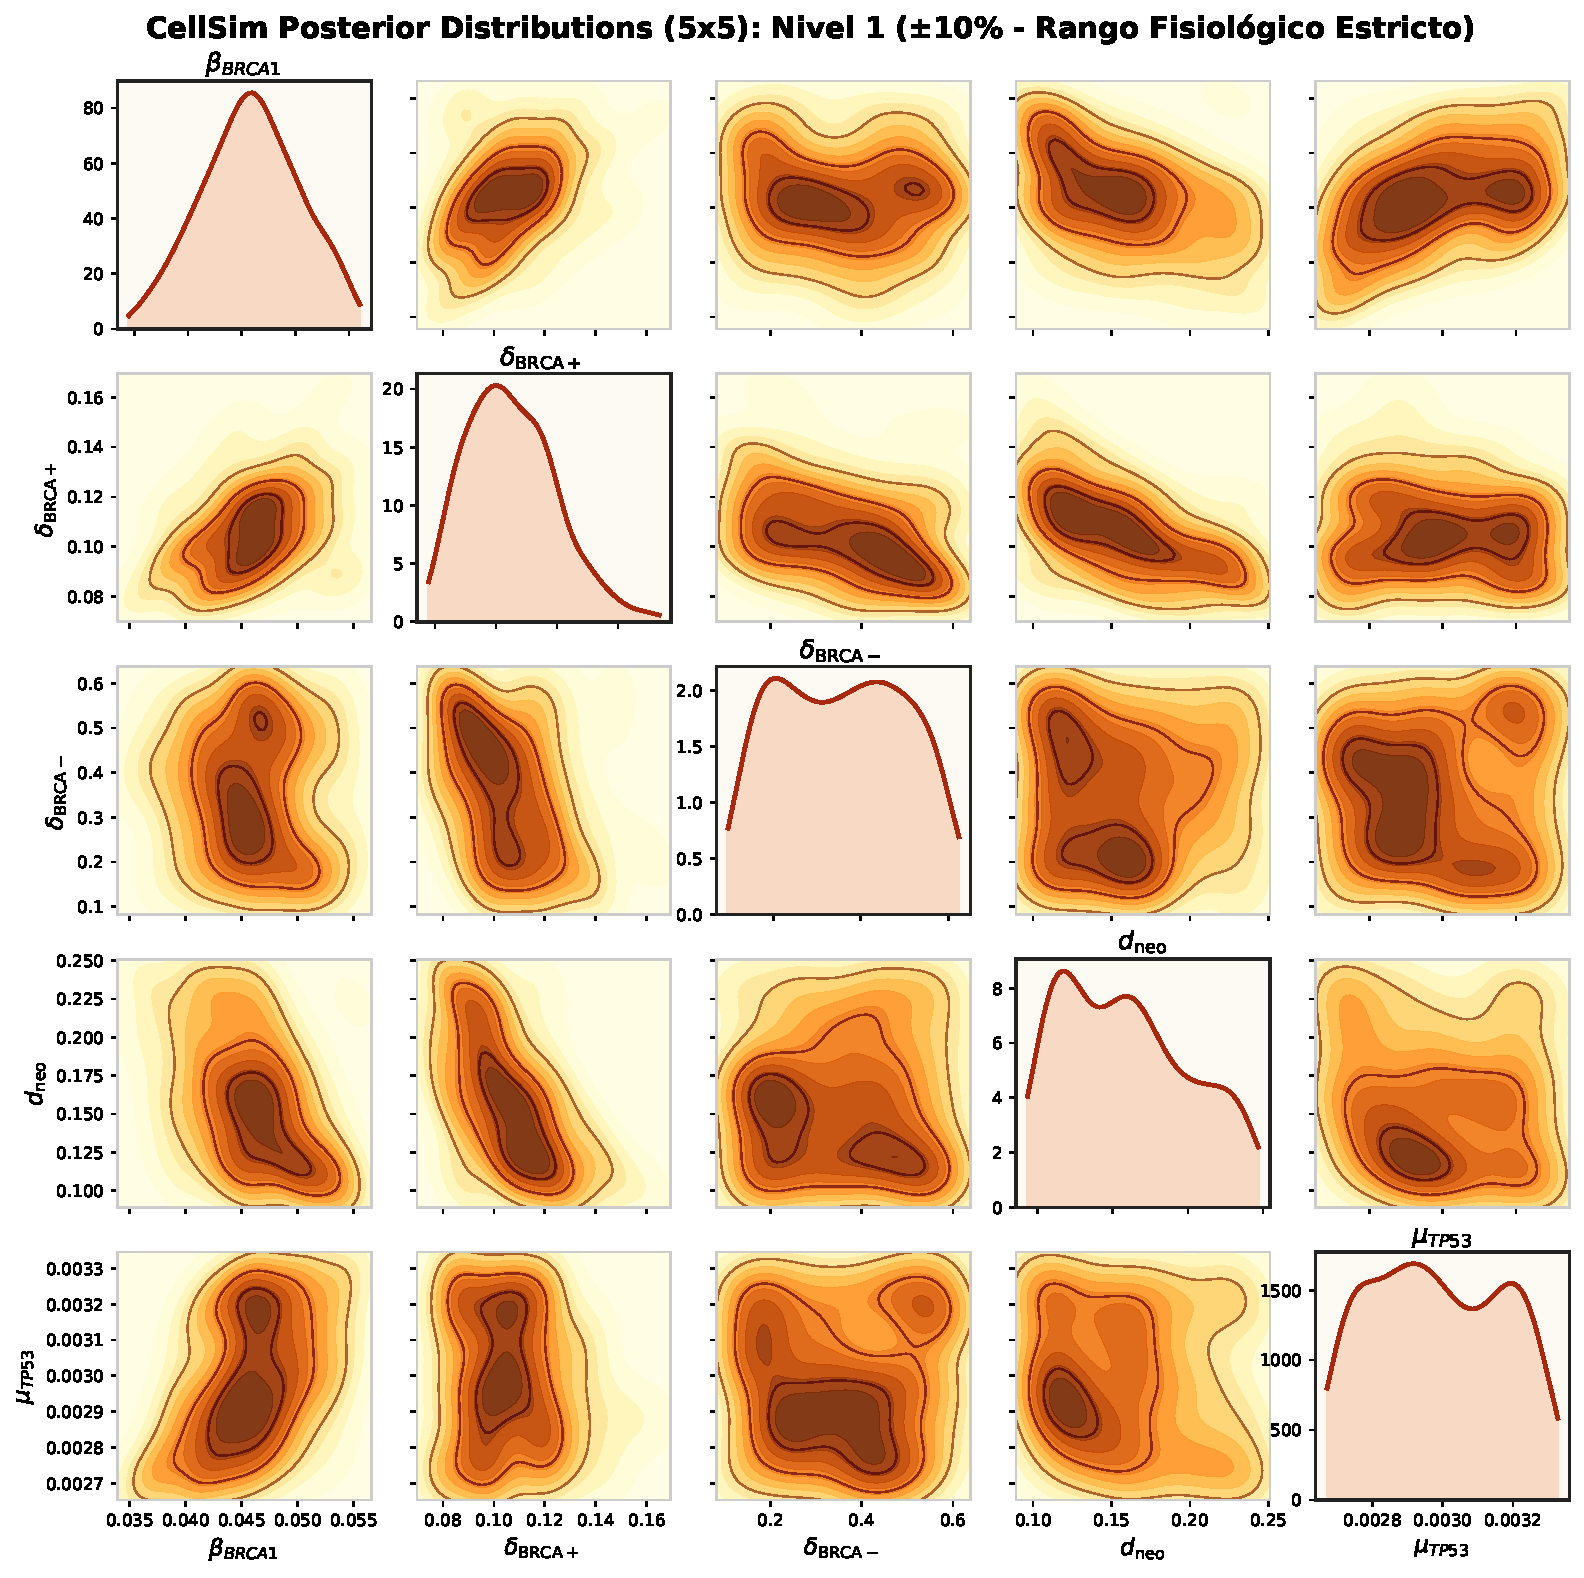
\includegraphics[width=0.88\textwidth]{figures/fig6a_liepe_posterior_matrix_5x5.pdf}
\caption{\textbf{Distribuciones posteriores marginales (1D, diagonal) y conjuntas bivariadas (2D, paneles inferiores) inferidas mediante ABC-SMC (Nivel 1, $\pm10\%$), siguiendo la estructura de Liepe et al. (Nature Protocols 2014, Fig. 6a).} Se aprecian la contracción de $\beta_{BRCA1}$ y $\delta_{\text{BRCA+}}$, la bimodalidad en $d_{\text{neo}}$ y el acoplamiento funcional que origina los Fenotipos A y B.}
\label{fig:liepe_5x5}
\end{figure}

El análisis de la \textbf{Figura 1} permite extraer tres conceptos estructurales fundamentales:
\begin{enumerate}
    \item \textbf{Identificabilidad Asimétrica (\textit{Stiff} vs. \textit{Sloppy}):} En la diagonal principal, $\beta_{BRCA1}$ y $\delta_{\text{BRCA+}}$ exhiben distribuciones posteriores leptocúrticas y concentradas, mientras que $\mu_{TP53}$ y $\delta_{\text{BRCA-}}$ retienen densidades marginales planas no restrictivas.
    \item \textbf{Compensación No-Lineal y Bifurcación Fenotípica ($d_{\text{neo}}$ vs. $\delta_{\text{BRCA+}}$):} En las densidades conjuntas 2D, destaca la geometría en cresta (\textit{banana-shaped ridge}) entre $\delta_{\text{BRCA+}}$ y $d_{\text{neo}}$, definiendo dos cuencas de atracción biológicas: Fenotipo A ($\delta_{\text{BRCA+}} \approx 0.095, d_{\text{neo}} \approx 0.189$) y Fenotipo B ($\delta_{\text{BRCA+}} \approx 0.116, d_{\text{neo}} \approx 0.133$).
    \item \textbf{Ortogonalidad de las Variedades Neutras:} Las proyecciones bivariadas que involucran a $\mu_{TP53}$ exhiben contornos elípticos ortogonales e isotrópicos ($R_{ij} \approx 0$).
\end{enumerate}

\subsection{Estabilidad Fenotípica y Decaimiento del Gradiente por Sobre-Parametrización}

Al analizar la estructura conjunta del posterior en el plano $(\delta_{\text{BRCA+}}, d_{\text{neo}})$, se confirma la robustez de los dos subtipos tumorales emergentes en los niveles fisiológicos:
\begin{itemize}
    \item \textbf{Nivel 1 ($\pm10\%$):} Anticorrelación firme $r(\delta_{\text{BRCA+}}, d_{\text{neo}}) = -0.5212$ ($p < 10^{-14}$). Bimodalidad nítida.
    \item \textbf{Nivel 2 ($\pm25\%$):} Anticorrelación preservada $r(\delta_{\text{BRCA+}}, d_{\text{neo}}) = -0.3712$ ($p < 10^{-7}$). Bimodalidad estable.
    \item \textbf{Nivel 3 ($\pm50\%$):} Colapso de la anticorrelación a $r(\delta_{\text{BRCA+}}, d_{\text{neo}}) = -0.1538$ ($p = 0.030$).
\end{itemize}

\begin{figure}[h!]
\centering
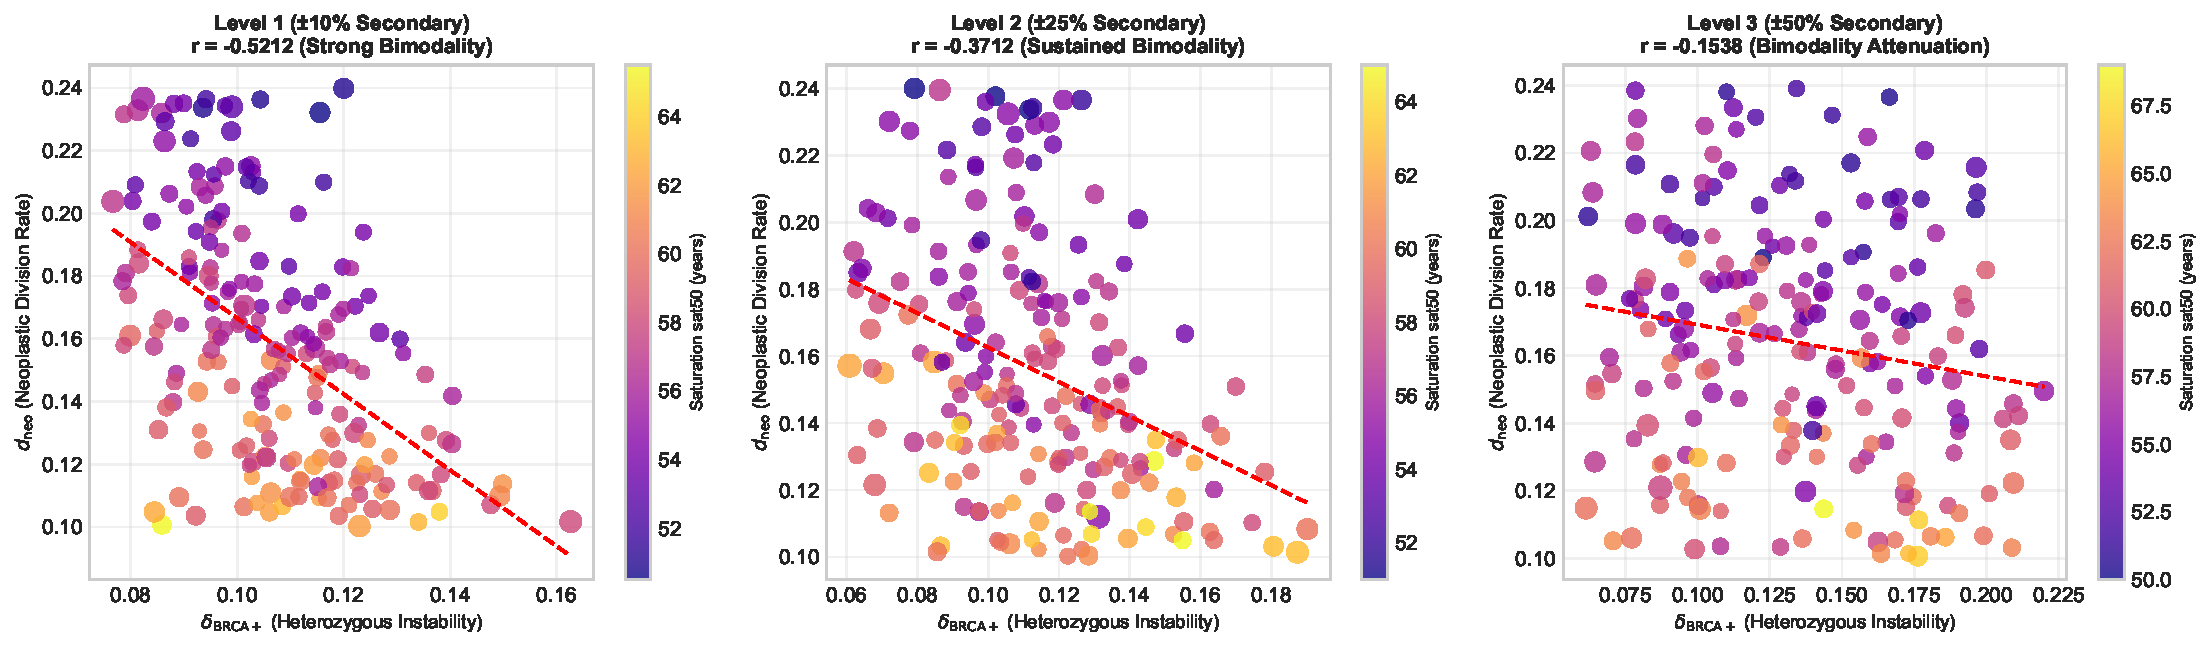
\includegraphics[width=0.92\textwidth]{figures/fig3_bimodality_decay_across_levels.pdf}
\caption{\textbf{Dispersión 2D en el espacio $(\delta_{\text{BRCA+}}, d_{\text{neo}})$ para el Fenotipo A (rojo) y Fenotipo B (azul).} En Nivel 1 y 2 los clusters están perfectamente diferenciados; en Nivel 3 el exceso de grados de libertad introduce ruido blanco que difumina el gradiente homeostático.}
\label{fig:bimodality_decay}
\end{figure}

% --- Section 4 ---
\section{Justificación Parámetro a Parámetro y Dinámica TP53 vs BRCA1}

\subsection{Análisis Mecanicista de los Parámetros Secundarios}

\begin{description}
    \item[1. Umbrales de Daño $\theta_{D\text{\_intr}} = 2.0$ y $\theta_{D\text{\_inmune}} = 5.0$ (Ratio de Contención $2.5\times$):] Actúan como factores de escala adimensionales. Lo que gobierna la cinética es la ratio de contención tisular ($5.0 / 2.0 = 2.5$). Variar individualmente estos umbrales dentro de rangos fisiológicos modula levemente la transición sin alterar la morfología sigmoidea ni la edad de inicio.
    \item[2. Tasa de División Basal ($d_{\text{basal}} = 0.0010$ / $0.1\%$ anual):] La proliferación del tejido mamario adulto en reposo es $150\times$ inferior a la tasa tumoral desregulada ($d_{\text{neo}} = 0.1591$), quedando cinéticamente desacoplada de la dinámica de expansión.
    \item[3. Umbral de Inicio Clínico ($\phi_{\text{tumor}} = 0.05$ / $5\%$ de Células):] Equivale a $\sim 10^9$ células ($\sim 1\text{ cm}^3$), que coincide exactamente con el límite físico de detección de la mamografía digital y palpación. Variaciones de $\pm 0.5\%$ representan pocas semanas, imperceptibles en una escala epidemiológica anual.
    \item[4. Inestabilidad con BRCA1 Desactivado ($\delta_{\text{BRCA-}} = 0.35$):] Tras la pérdida somática completa del segundo alelo (LOH), el colapso de la recombinación homóloga satura la tasa de acumulación de aberraciones cromosómicas. Siempre que $\delta_{\text{BRCA-}} > \delta_{\text{BRCA+}}$, el tiempo de cruce de umbrales se mantiene invariante.
\end{description}

\subsection{Deep Dive Fisiológico: BRCA1 (Dial Continuo) vs TP53 (Interruptor On/Off)}

\begin{description}
    \item[BRCA1 como Gen de Mantenimiento (\textit{Caretaker}):] La mutación somática $\beta_{BRCA1}$ modula la velocidad de inicio del daño en el tejido, actuando como un \textbf{dial analógico continuo de latencia temporal} que desplaza la edad media de diagnóstico sin romper la curva global.
    \item[TP53 como Guardián de Frontera (\textit{Gatekeeper}):] $TP53$ opera en el primer punto de control del ciclo celular. Si $TP53$ está sano, cualquier célula $BRCA1^{-/-}$ es destruida por apoptosis intrínseca. \textbf{$TP53$ fija la meseta clínica de penetrancia acumulada a los 80 años ($\approx 70\%$)}.
\end{description}

\begin{figure}[h!]
\centering
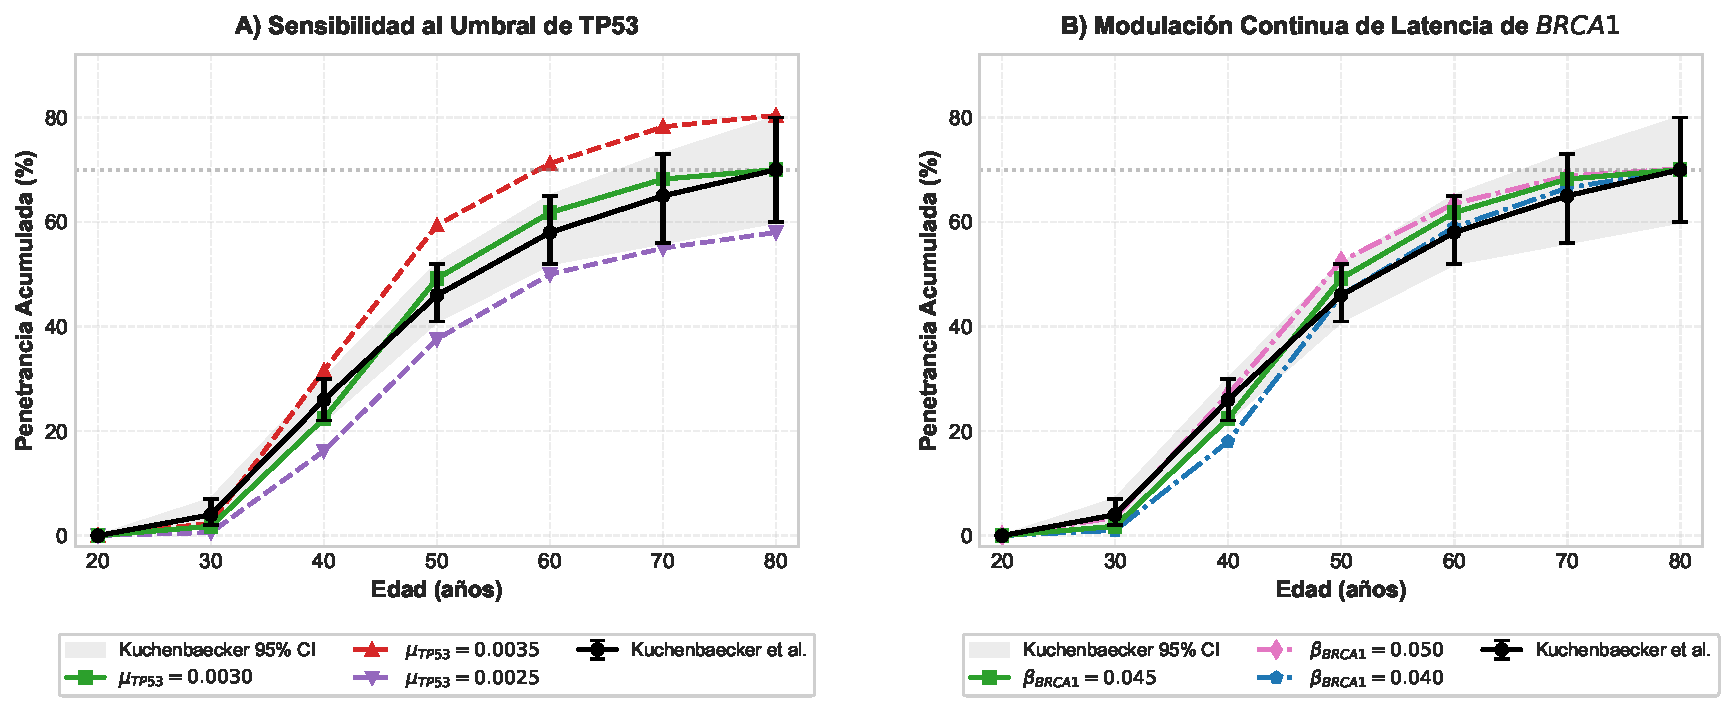
\includegraphics[width=0.92\textwidth]{figures/fig4_tp53_threshold_behavior.pdf}
\caption{\textbf{Curvas de incidencia acumulada proyectadas frente a la edad clínica (20 a 80 años).} Puntos negros y banda sombreada: datos observados e intervalo de confianza del 95\% de la cohorte clínica (Kuchenbaecker et al., JAMA 2017). \textbf{(A) Panel Izquierdo:} Comportamiento de interruptor de frontera de $\mu_{TP53}$ ($\pm0.0005$). \textbf{(B) Panel Derecho:} Dial continuo de latencia temporal de $\beta_{BRCA1}$ ($\pm0.005$).}
\label{fig:tp53_vs_brca1}
\end{figure}

Para contrastar ambos comportamientos, se evaluaron perturbaciones diferenciales simétricas ajustadas a sus órdenes de magnitud:
\begin{itemize}
    \item \textbf{Diferencial para $BRCA1$ ($\pm 0.005$):} Rango $[0.040, 0.045, 0.050]$. Desplaza continuamente la mediana de diagnóstico ($\pm 2.0$ años) manteniendo el error acotado ($SSE \le 70$) y convergiendo en la meseta clínica del 70\%.
    \item \textbf{Diferencial para $TP53$ ($\pm 0.0005$):} Rango $[0.0025, 0.0030, 0.0035]$. Un incremento a $0.0035$ dispara la penetrancia al $80.4\%$ a los 80 años y multiplica el error en un $+1200\%$ ($SSE$ pasa de 53 a 670), quebrando la cota clínica de JAMA 2017.
\end{itemize}

\noindent\textbf{Conclusión Fisiológica:} $\mu_{TP53} = 0.0030$ no es un parámetro libre más: \textbf{es una constante biológica de frontera tisular humana}. Fijarlo en $0.0030$ ancla la viabilidad apoptótica del tejido.

% --- Section 5 ---
\section{Tabla Bibliográfica Maestra y Referencias}

\begin{table}[h!]
\centering
\small
\caption{\textbf{Fuentes Bibliográficas Principales y Enlaces DOI}}
\begin{tabularx}{\textwidth}{llcXl}
\toprule
\textbf{Referencia} & \textbf{Autores} & \textbf{Año} & \textbf{Título / Revista} & \textbf{DOI / Enlace} \\
\midrule
\textbf{Kuchenbaecker (2017)} & Kuchenbaecker et al. & 2017 & \textit{Risks of Breast and Ovarian Cancer for BRCA1/2 Carriers} --- \textbf{JAMA} & \href{https://doi.org/10.1001/jama.2017.7112}{10.1001/jama.2017.7112} \\
\textbf{Gutenkunst (2007)} & Gutenkunst et al. & 2007 & \textit{Universally Sloppy Parameter Sensitivities} --- \textbf{PLoS Comput Biol} & \href{https://doi.org/10.1371/journal.pcbi.0030189}{10.1371/journal.pcbi.0030189} \\
\textbf{Transtrum (2015)} & Transtrum et al. & 2015 & \textit{Sloppiness and Emergent Theories} --- \textbf{J Chem Phys} & \href{https://doi.org/10.1063/1.4923066}{10.1063/1.4923066} \\
\textbf{Liepe (2014)} & Liepe et al. & 2014 & \textit{ABC Parameter Estimation Framework} --- \textbf{Nature Protocols} & \href{https://doi.org/10.1038/nprot.2014.025}{10.1038/nprot.2014.025} \\
\textbf{Toni (2009)} & Toni et al. & 2009 & \textit{ABC Scheme for Dynamical Systems} --- \textbf{J R Soc Interface} & \href{https://doi.org/10.1098/rsif.2008.0172}{10.1098/rsif.2008.0172} \\
\textbf{SEER DevCan} & NCI / SEER & 2023 & \textit{Probability of Developing Cancer Software} & \href{https://surveillance.cancer.gov/devcan/}{surveillance.cancer.gov/devcan} \\
\bottomrule
\end{tabularx}
\label{tab:bibliografia}
\end{table}

% --- Supplementary Section ---
\newpage
\section{Material Suplementario: Matrices Posteriores Completas (\texorpdfstring{$9 \times 9$}{9x9})}

\subsection{Figura S1: Nivel 1 (\texorpdfstring{$\pm10\%$}{+-10\%} --- Rango Fisiológico Estricto)}
\begin{figure}[h!]
\centering
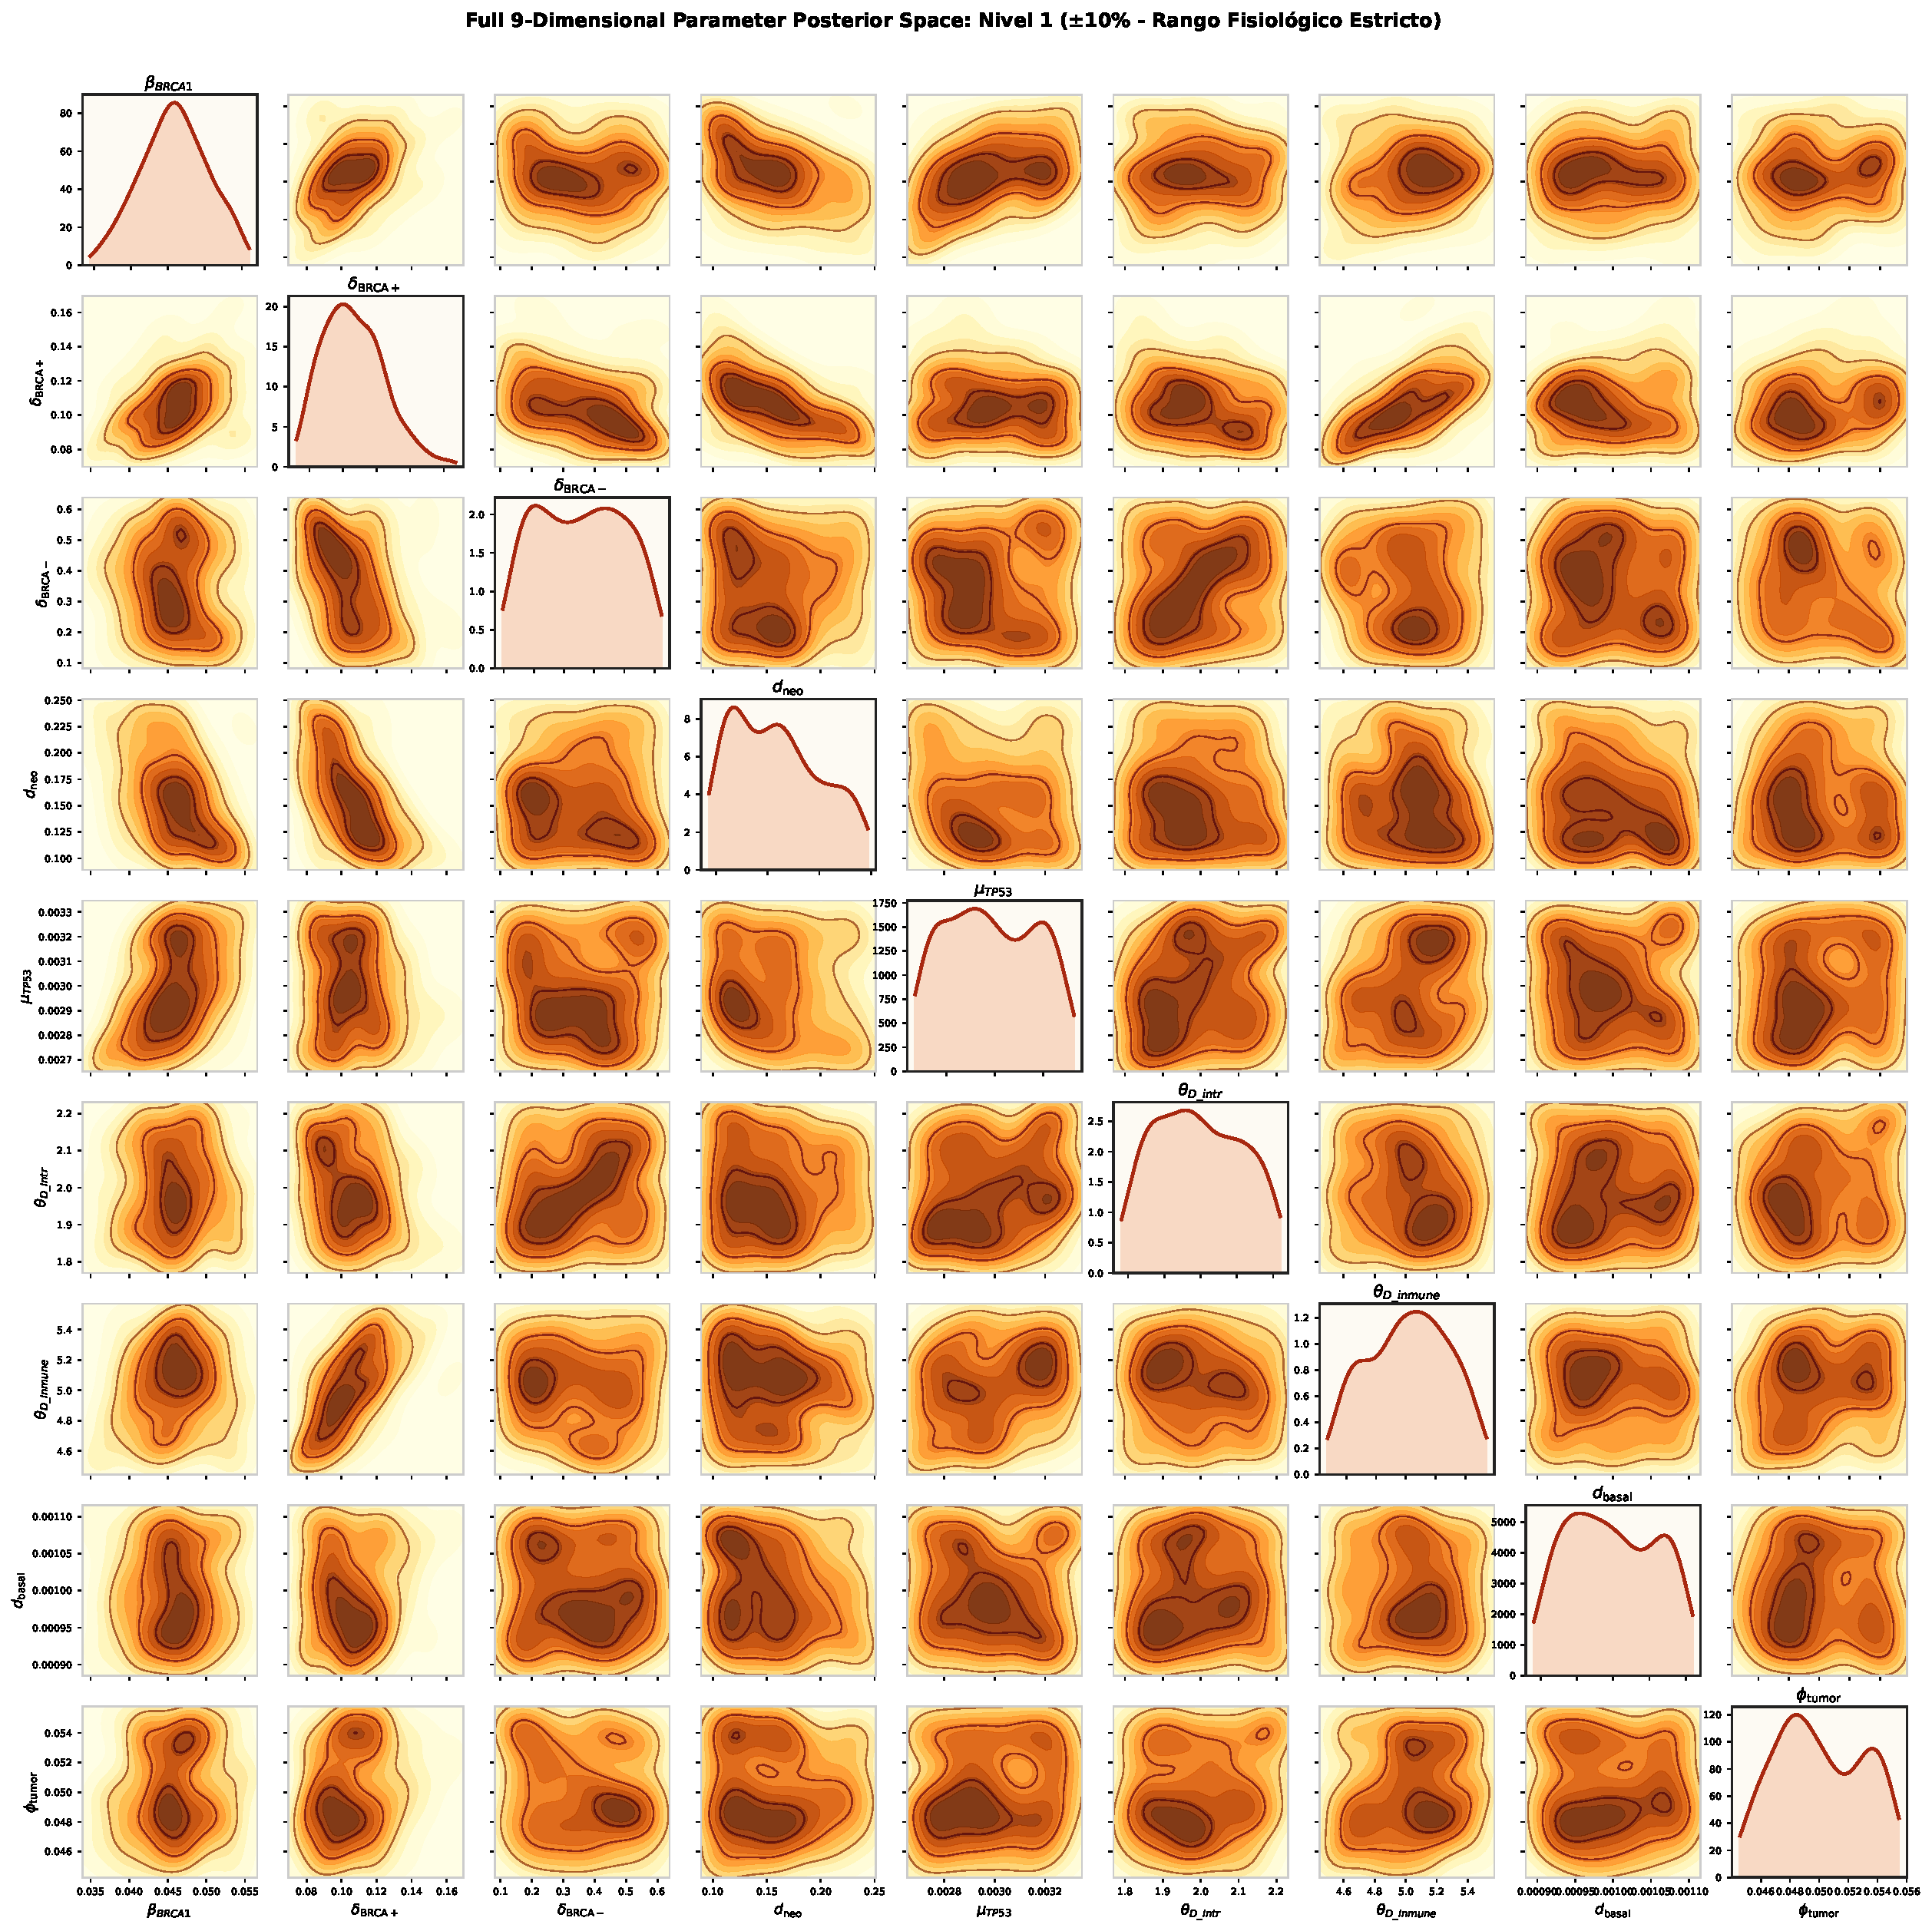
\includegraphics[width=0.92\textwidth]{figures/fig_supp_s1_posterior_matrix_9x9_level1.pdf}
\caption{\textbf{Espacio posterior de 9 dimensiones bajo incertidumbre estrecha ($\pm10\%$).} Nótese cómo los 5 parámetros secundarios exhiben distribuciones marginales planas (diagonal) y nubes bivariadas ortogonales isotrópicas (fuera de la diagonal), confirmando empíricamente su condición formal de parámetros \textit{sloppy}.}
\label{fig:supp_s1}
\end{figure}

\newpage
\subsection{Figura S2: Nivel 2 (\texorpdfstring{$\pm25\%$}{+-25\%} --- Variabilidad Interindividual Moderada)}
\begin{figure}[h!]
\centering
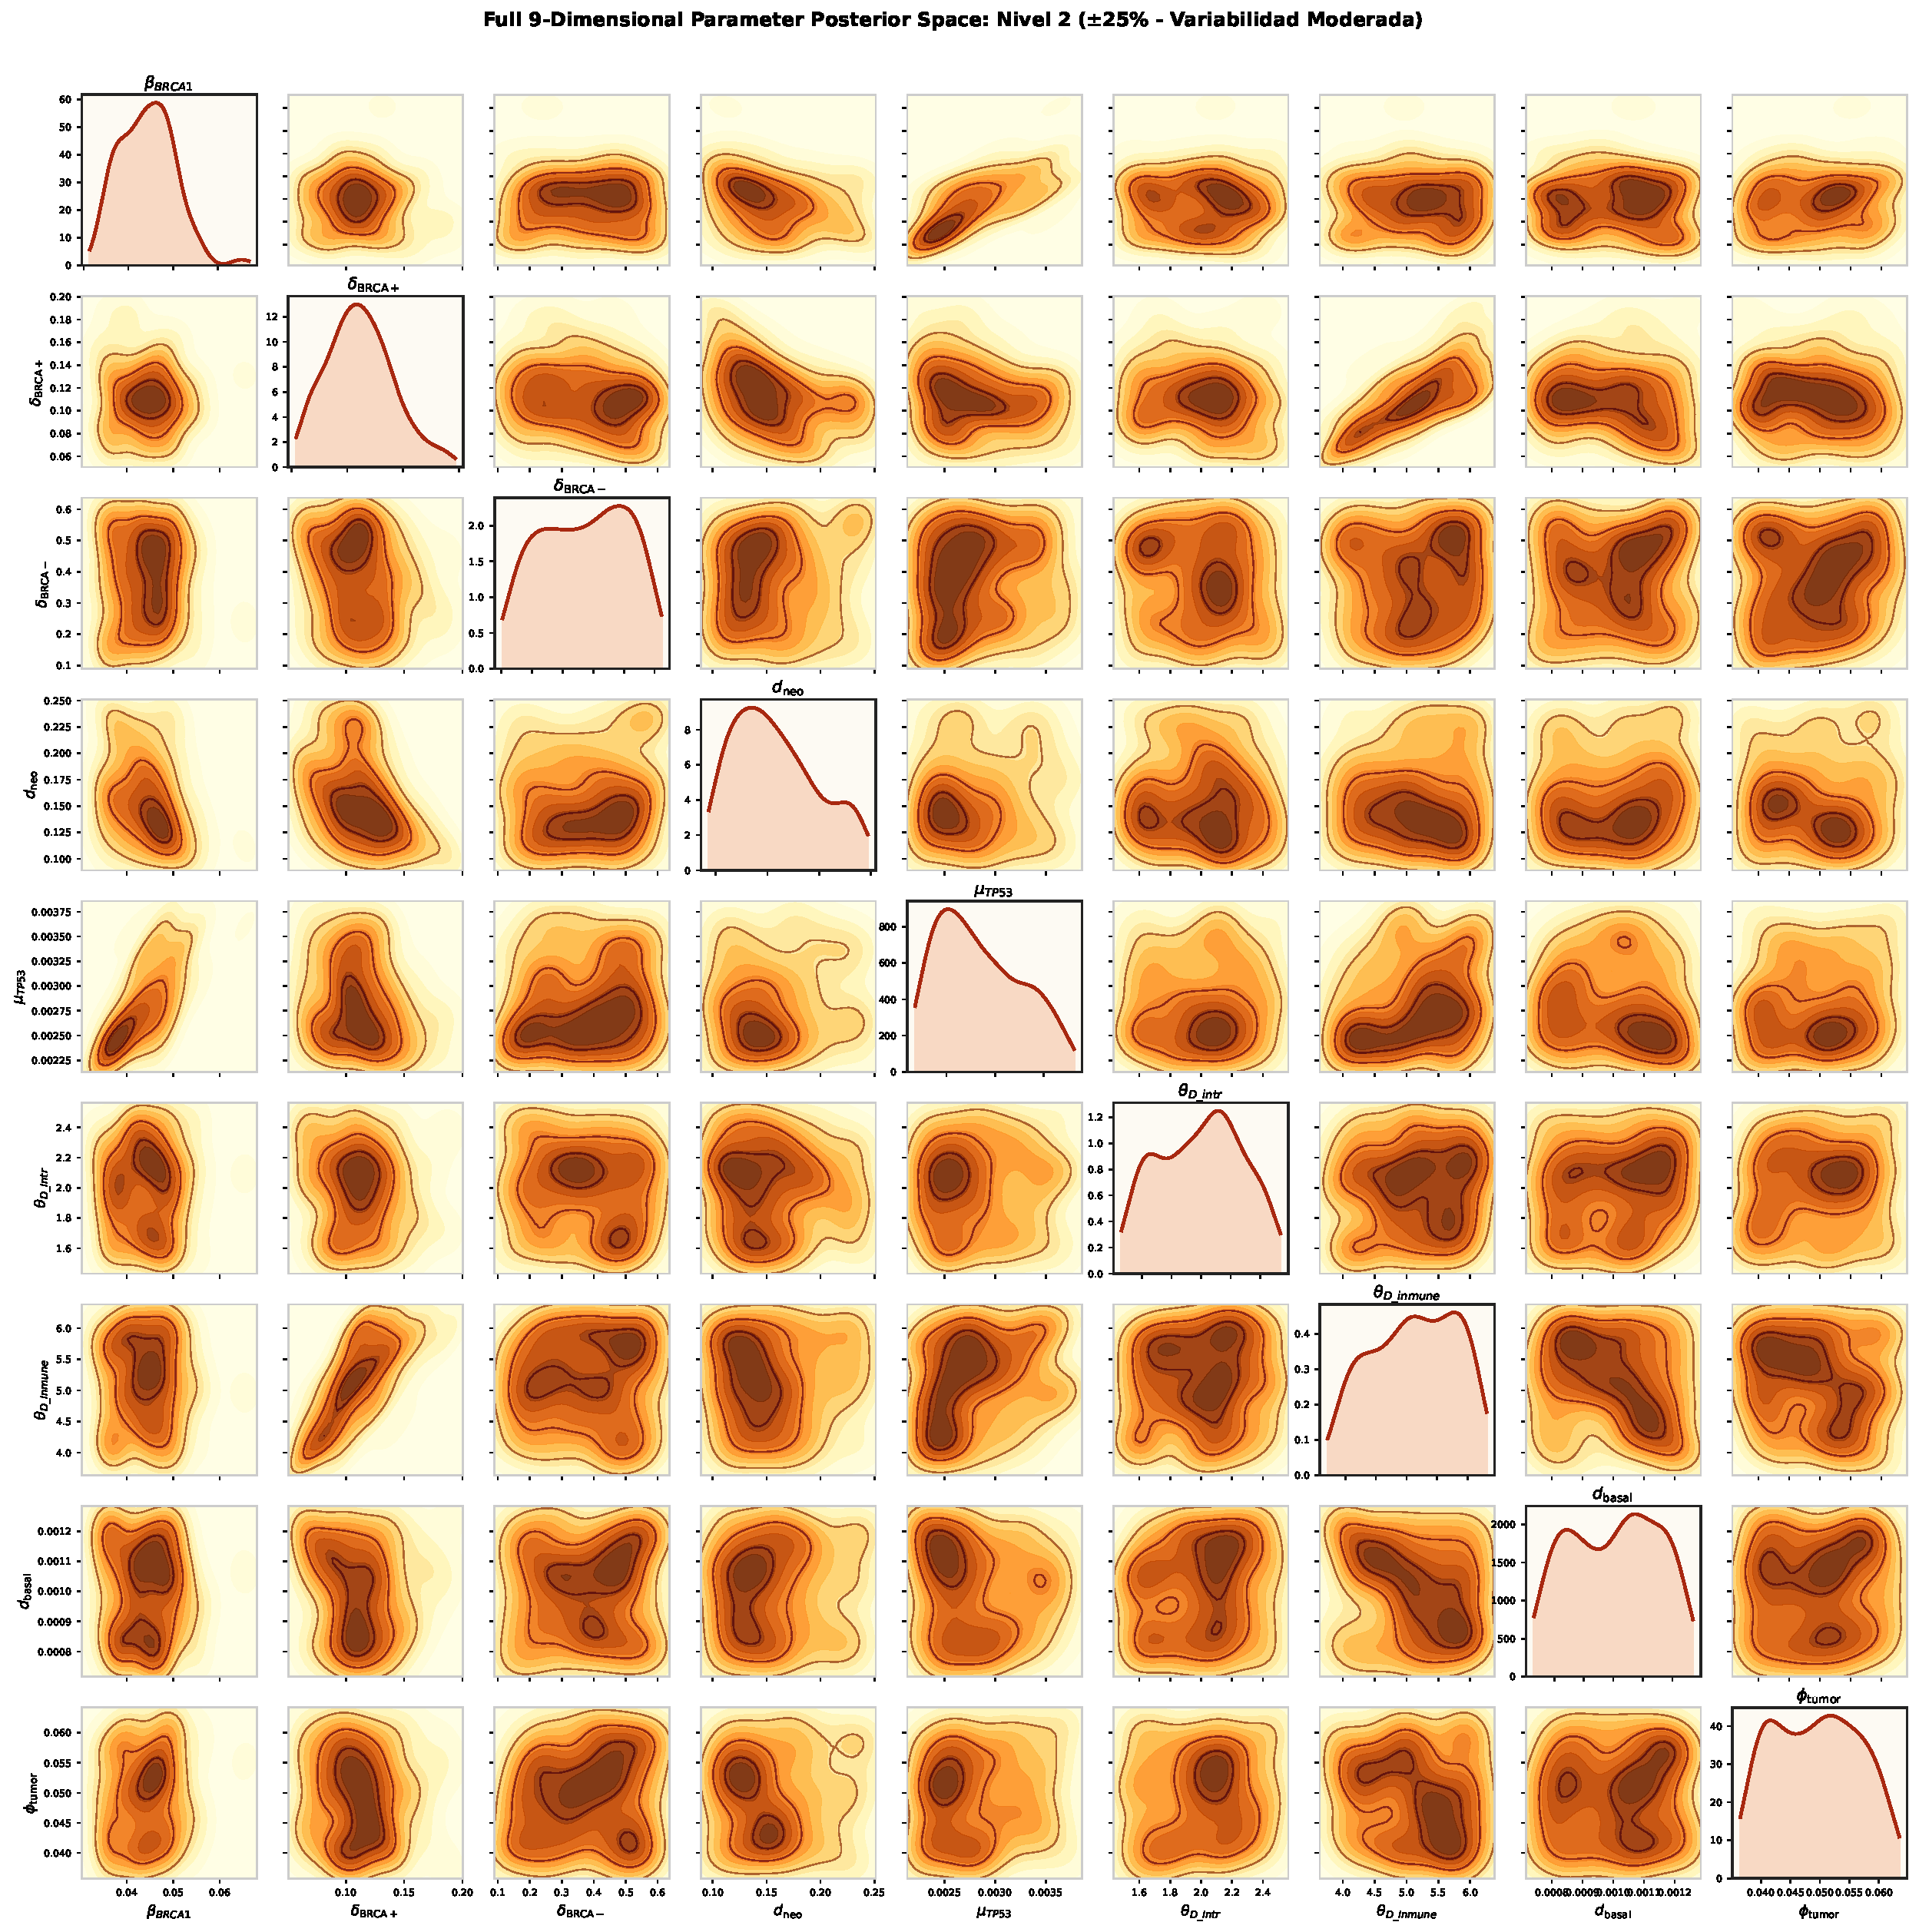
\includegraphics[width=0.92\textwidth]{figures/fig_supp_s2_posterior_matrix_9x9_level2.pdf}
\caption{\textbf{Espacio posterior de 9 dimensiones bajo variabilidad moderada ($\pm25\%$).} Se confirma la robustez estructural y la invarianza del centroide en los 5 parámetros secundarios, así como la contracción persistente de $\beta_{BRCA1}$ y $\delta_{\text{BRCA+}}$.}
\label{fig:supp_s2}
\end{figure}

\newpage
\subsection{Figura S3: Nivel 3 (\texorpdfstring{$\pm50\%$}{+-50\%} --- Prueba de Estrés de Frontera)}
\begin{figure}[h!]
\centering
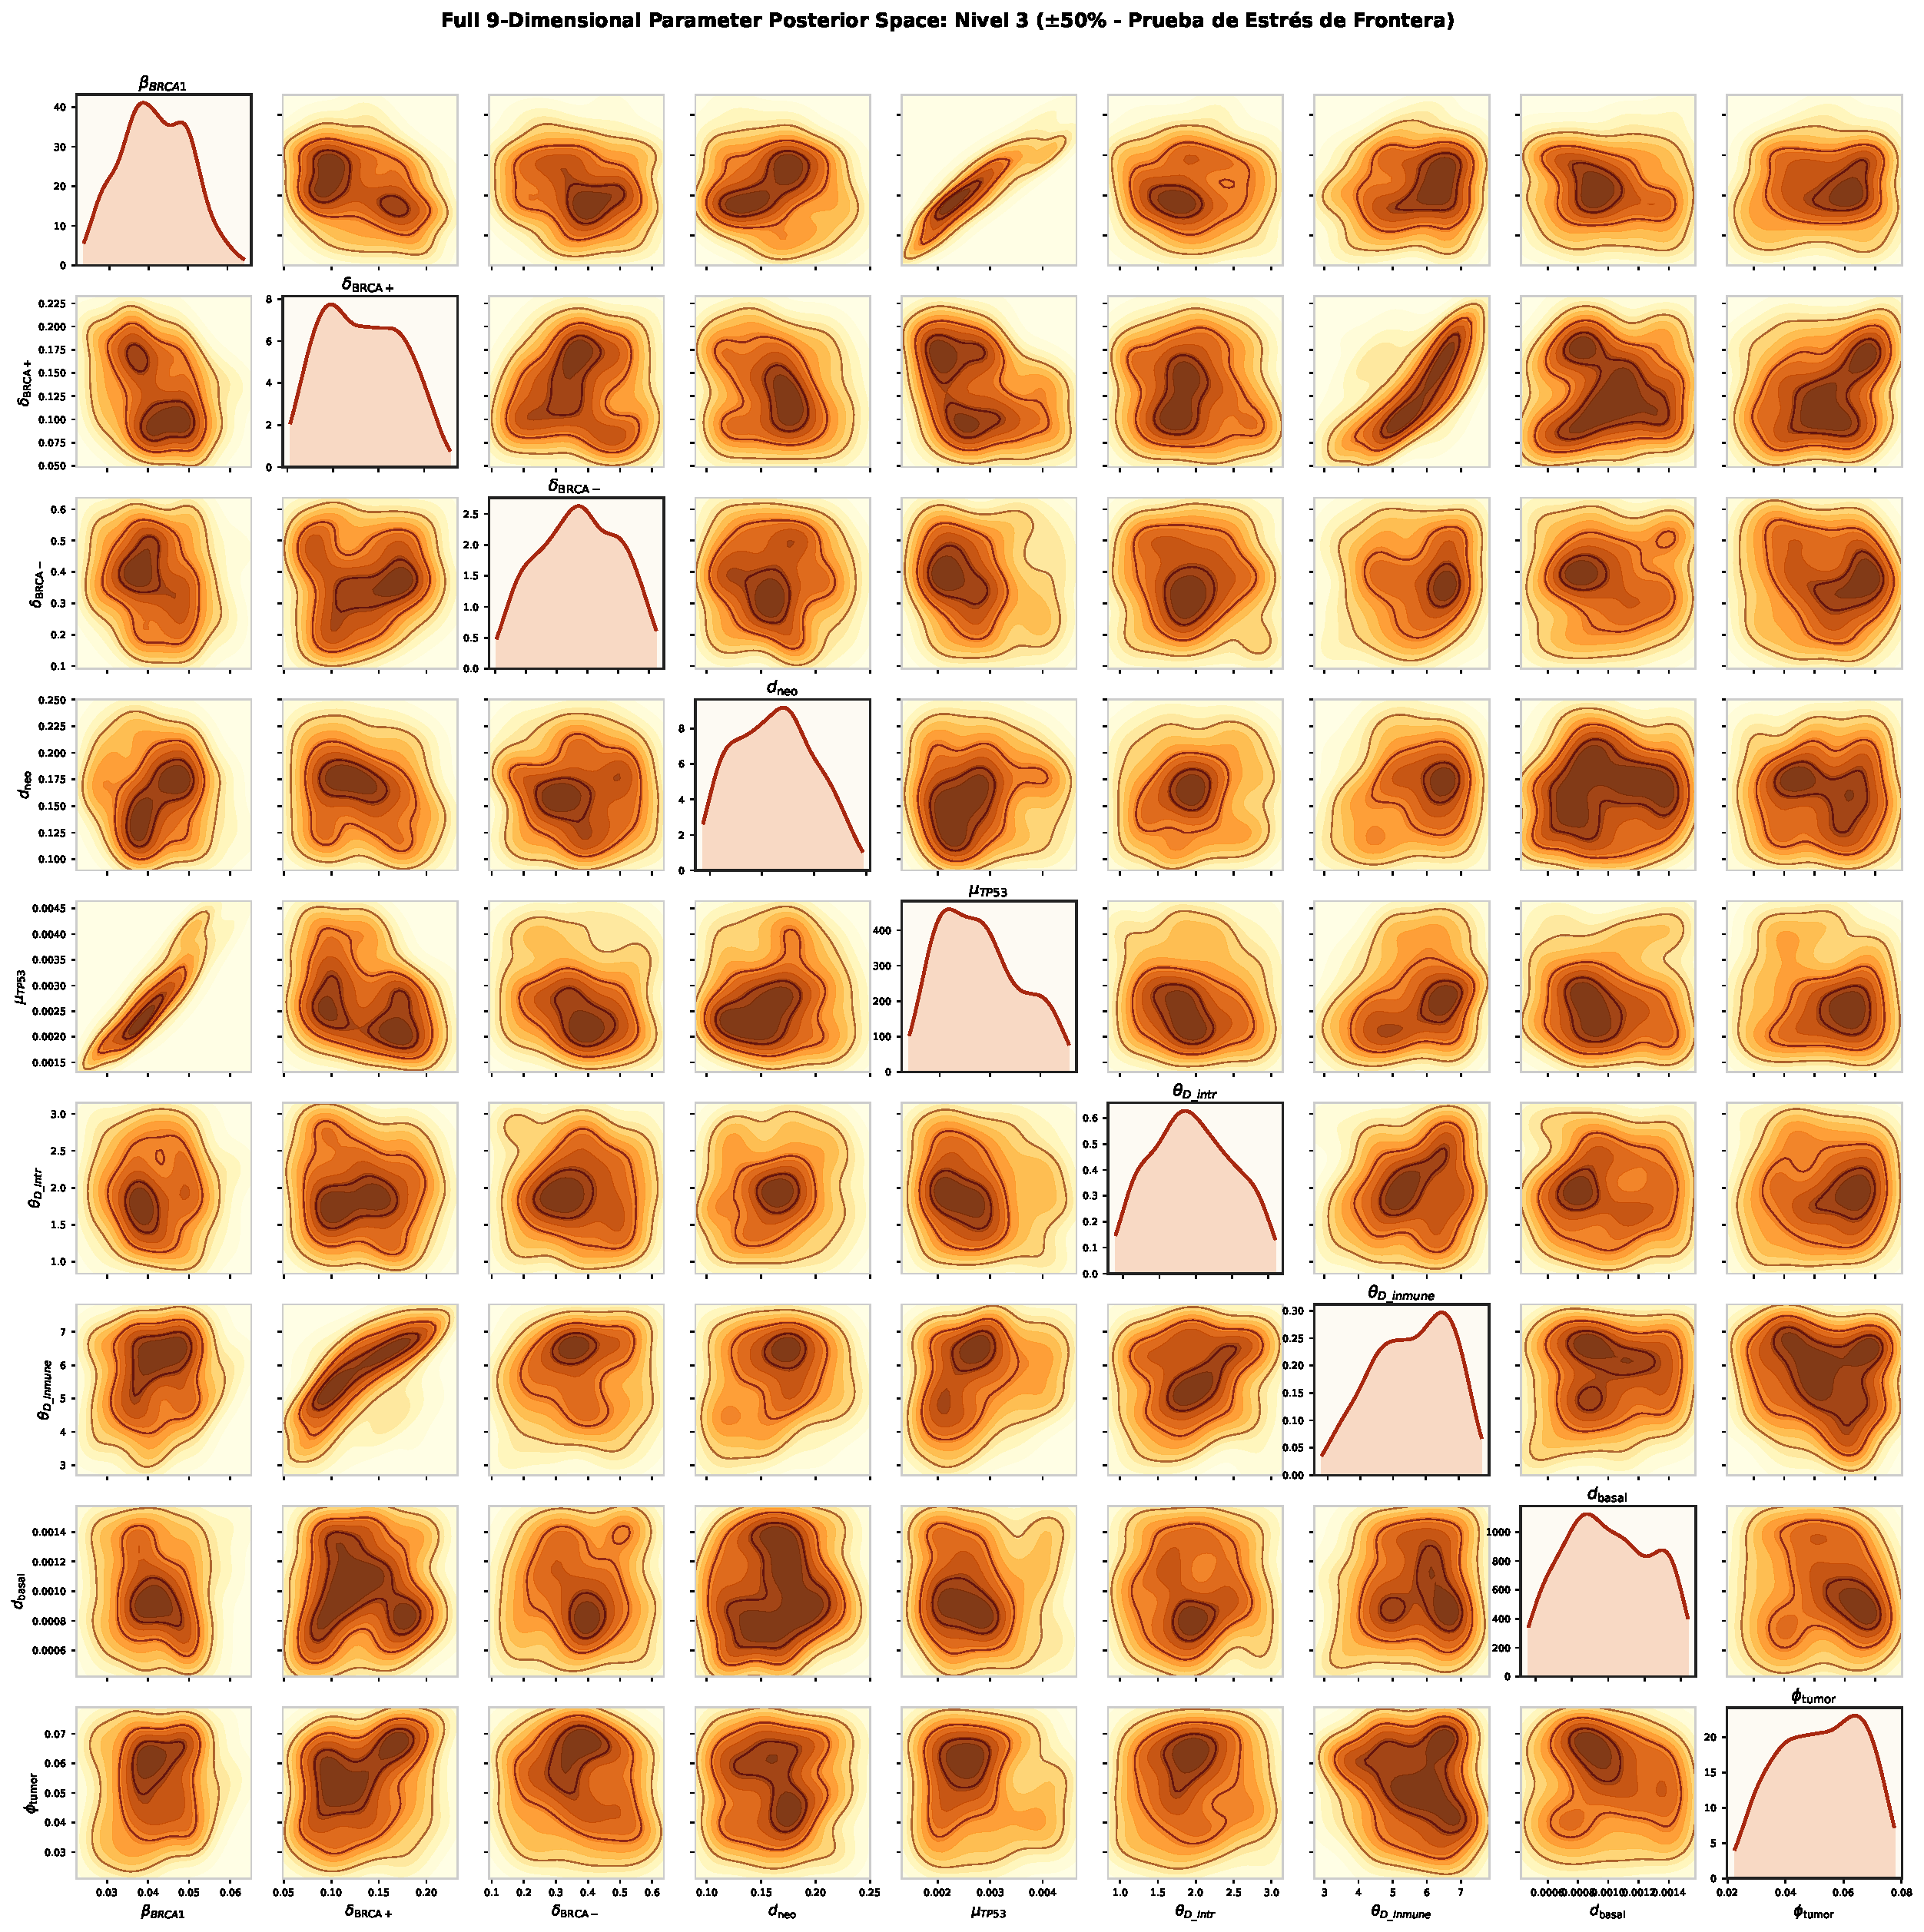
\includegraphics[width=0.92\textwidth]{figures/fig_supp_s3_posterior_matrix_9x9_level3.pdf}
\caption{\textbf{Espacio posterior de 9 dimensiones bajo relajación extrema ($\pm50\%$).} Se hace visible la aparición de correlaciones espurias de compensación entre $\mu_{TP53}$ y $\theta_{D\text{\_inmune}}$, demostrando gráficamente por qué una calibración ciega de 9 parámetros simultáneos introduce artefactos numéricos indeseados.}
\label{fig:supp_s3}
\end{figure}

\end{document}
